\section{\label{sec:classification}Classification of space groups}

\begin{figure}[htb]
\centering
\begin{tikzpicture}
  \tikzset{nodestyle/.style={draw}};

  \node[nodestyle] (family) {6 crystal families (Sec.~\ref{sec:crystal-family})};

  \node[nodestyle, below left=0.5cm of family] (lattice-system) {7 lattice systems (Sec.~\ref{sec:lattice-system})};
  \node[nodestyle, below=1cm of lattice-system] (bravais-class) {14 Bravais classes (Sec.~\ref{sec:bravais-class})};

  \node[nodestyle, below right=0.5cm of family] (crystal-system) {7 crystal systems (Sec.~\ref{sec:crystal-system})};
  \node[nodestyle, below=1cm of crystal-system] (geometric-class) {32 geometric crystal classes (Sec.~\ref{sec:geometric-class})};

  \node[nodestyle, below=3cm of family] (arithmetic-class) {73 arithmetic crystal classes (Sec.~\ref{sec:arithmetic-crystal-class})};
  \node[nodestyle, below=1cm of arithmetic-class] (affine) {219 affine space-group types (Sec.~\ref{sec:space-group-type})};
  \node[nodestyle, below=1cm of affine] (spacegroup) {230 crystallographic space-group types (Sec.~\ref{sec:space-group-type})};

  \draw (family) -- (lattice-system);
  \draw (family) -- (crystal-system);

  \draw (lattice-system) -- (bravais-class);
  \draw (crystal-system) -- (geometric-class);

  \draw (bravais-class) -- (arithmetic-class);
  \draw (geometric-class) -- (arithmetic-class);

  \draw (arithmetic-class) -- (affine);
  \draw (affine) -- (spacegroup);
\end{tikzpicture}
\caption{Classification of space groups}
\label{fig:space_group_classification}
\end{figure}

We classify space groups in three dimensions (see Fig.~\ref{fig:space_group_classification} for the hierarchy of the classifications).

\subsection{\label{sec:space-group-type}Affine space-group type and space-group type}

It is natural to identify two space groups that are transformed into another by changing coordinate systems.
\begin{screen}
  \begin{defn}[affine space-group type]
    Two space groups $\mathcal{G}, \mathcal{G}'$ belong to the same \term{affine space-group type} if they are conjugate by some affine mapping $(\bm{P}, \bm{p}) \in \mathcal{A}_{3}$ such that $(\bm{P}, \bm{p})^{-1} \mathcal{G} (\bm{P}, \bm{p}) = \mathcal{G}'$.
    These space groups are also called \term{affinely equivalent}.
  \end{defn}
\end{screen}
Note that we do not restrict the domain of $(\bm{P}, \bm{p})$ in the definition of the affine space-group type into $\mathcal{E}_{3}$ because we would like to identify different crystal structures with the same matrix representations of symmetry operations.

It is nontrivial fact that affine equivalence completely identifies the isomorphism of space groups.

\begin{screen}
  \begin{them}[Bieberbach]
    Two space groups are isomorphic if and only if they belong to the same affine type.
  \end{them}
\end{screen}

In crystallography, a tighter classification of space groups is often used.
That is, orientation-preserving affine mapping is only considered in transformations of coordinates systems\footnote{
  Some people indicate ``space groups'' as space-group types in their terminology.
  I think the clear distinction between space groups and space-group types makes our lives easier.
}.

\begin{screen}
  \begin{defn}[space-group type]
    Two space groups $\mathcal{G}, \mathcal{G}'$ belong to the same \term{(crystallographic) space-group type} if they are conjugate by some orientation-preserving affine mapping $(\bm{P}, \bm{p}) \in \mathcal{A}^{+}_{3}$ such that $(\bm{P}, \bm{p})^{-1} \mathcal{G} (\bm{P}, \bm{p}) = \mathcal{G}'$, where orientation-preserving affine mapping is an affine mapping whose linear part is positive,
    \begin{align}
      \mathcal{A}^{+}_{n} \coloneqq \set{ \begin{pmatrix} \bm{W} & \bm{w} \\ \bm{0}^{\top} & 1 \end{pmatrix} }{ \bm{W} \in \mathrm{GL}(n, \mathbb{R}), \det \bm{W} > 0, \bm{w} \in \mathbb{R}^{n} }.
    \end{align}
  \end{defn}
\end{screen}

A pair of affine space-groups types that belong to the different crystallographic space-group types are called \term{enantiomorphic pair}.
For example, there are 11 enantiomorphic pairs in three dimensions as Table.~\ref{table:enantiomorphic-pairs-3d}.

\begin{table}[htb]
  \centering
  \caption{Enantiomorphic pairs in space groups}
  \label{table:enantiomorphic-pairs-3d}
  \begin{tabular}[h]{cc}
    \hline\hline
    $P 4_{1}$ (76)         & $P 4_{3}$ (78) \\
    $P 4_{1} 2 2$ (91)     & $P 4_{3} 2 2$ (95) \\
    $P 4_{1} 2_{1} 2$ (92) & $P 4_{3} 2_{1} 2$ (96) \\
    $P 3_{1}$ (144)        & $P 3_{2}$ (145) \\
    $P 3_{1} 1 2$ (151)    & $P 3_{2} 1 2$ (153) \\
    $P 3_{1} 2 1$ (152)    & $P 3_{2} 2 1$ (154) \\
    $P 6_{1}$ (169)        & $P 6_{5}$ (173) \\
    $P 6_{2}$ (170)        & $P 6_{4}$ (172) \\
    $P 6_{1} 2 2$ (178)    & $P 6_{5} 2 2$ (179) \\
    $P 6_{2} 2 2$ (180)    & $P 6_{4} 2 2$ (181) \\
    $P 4_{3} 3 2$ (212)    & $P 4_{1} 3 2$ (213) \\
    \hline\hline
  \end{tabular}
\end{table}

\subsection{\label{sec:arithmetic-crystal-class}Arithmetic crystal class}

\begin{screen}
  \begin{defn}[arithmetic crystal class]
    Two subgroups of $\mathrm{GL}(3, \mathbb{Z})$, $\mathcal{P}$ and $\mathcal{P}'$, belong to the same \term{arithmetic crystal class} if they are conjugate by some unimodular matrix $\bm{P} \in \mathrm{SL}(3, \mathbb{Z})$ such that $\bm{P}^{-1} \mathcal{P} \bm{P} = \mathcal{P}'$.
    Two space groups $\mathcal{G}$ and $\mathcal{G}'$ with point groups $\mathcal{P}$ and $\mathcal{P}'$, both written with primitive basis vectors, belong to the same \term{arithmetic crystal class} if $\mathcal{P}$ and $\mathcal{P}'$ belong to the same arithmetic crystal class.
  \end{defn}
\end{screen}

The arithmetic crystal class forgets vector systems of space groups in Sec.~\ref{sec:vector_system}.
Therefore, the arithmetic crystal classes have a one-to-one correspondence with symmorphic space-group types.
There are \href{https://dictionary.iucr.org/Arithmetic_crystal_class}{73 arithmetic crystal classes} for space groups.
We mention that the transformation matrix $\bm{P}$ is restricted in $\mathrm{SL}(3, \mathbb{Z})$ (not $\mathrm{SL}(3, \mathbb{R})$) to preserve centerings of translation subgroup $\mathcal{T}(\mathcal{G})$, which we will explain in more detail in the example of the next section.

\subsection{\label{sec:geometric-class}Classification based on point group}

We consider classification based on a point group of a space group.

\begin{screen}
  \begin{defn}[geometric crystal class]
    Two subgroups of $\mathrm{GL}(3, \mathbb{Z})$, $\mathcal{P}$ and $\mathcal{P}'$, belong to the same \term{geometric crystal class} if they are conjugate by some invertible matrix $\bm{P} \in \mathrm{SL}(3, \mathbb{R})$ such that $\bm{P}^{-1} \mathcal{P} \bm{P} = \mathcal{P}'$.
    Two space groups $\mathcal{G}$ and $\mathcal{G}'$ with point groups $\mathcal{P}$ and $\mathcal{P}'$, respectively, belong to the same \term{geometric crystal class} if $\mathcal{P}$ and $\mathcal{P}'$ belong to the same geometric crystal class.
  \end{defn}
\end{screen}

There are 32 geometric crystal classes for space groups shown in Table~\ref{tab:crystal_system}.

Two space groups belong to the same \term{Laue class} if point groups obtained by their point group with inversions belong to the same geometric crystal class (Table~\ref{tab:laue_class}).

\begin{table}[htb]
  \centering
  \caption{Laue classes in space groups}
  \label{tab:laue_class}
  \begin{tabular}[h]{cc}
    \hline\hline
    Laue class       & Geometric crystal class \\ \hline
    $\overline{1}$   & $1$, $\overline{1}$ \\
    $2/m$            & $2$, $m$, $2/m$ \\
    $mmm$            & $222$, $2mm$, $mmm$ \\
    $\overline{3}$   & $3$, $\overline{3}$ \\
    $\overline{3}m$  & $32$, $3m$, $\overline{3}m$ \\
    $4/m$            & $4$, $\overline{4}$, $4/m$ \\
    $4/mmm$          & $422$, $\overline{4}2m$, $4mm$, $4/mmm$ \\
    $6/m$            & $6$, $\overline{6}$, $6/m$ \\
    $6/mmm$          & $622$, $\overline{6}2m$, $6mm$, $6/mmm$ \\
    $m\overline{3}$  & $23$, $m\overline{3}$ \\
    $m\overline{3}m$ & $432$, $\overline{4}32$, $m\overline{3}m$ \\
    \hline\hline
  \end{tabular}
\end{table}

\paragraph{Example: point groups of $P\overline{4}2m$ and $P\overline{4}m2$}

The point group of space-group type $P\overline{4}2m$ is generated from fourfold rotoinversion along the $c$ axis and twofold rotation along the $a$ axis,
\begin{align*}
  \overline{4}^{+}_{001}:
    \begin{pmatrix}
      0 & 1 & 0 \\
      -1 & 0 & 0 \\
      0 & 0 & -1 \\
    \end{pmatrix},
  2_{100}:
    \begin{pmatrix}
      1 & 0 & 0 \\
      0 & -1 & 0 \\
      0 & 0 & -1 \\
    \end{pmatrix}.
\end{align*}
On the other hand, the point group of space-group type $P\overline{4}m2$ is generated from fourfold rotoinversion along the $c$ axis and twofold rotation along the $[110]$ axis,
\begin{align*}
  \overline{4}^{+}_{001}:
    \begin{pmatrix}
      0 & 1 & 0 \\
      -1 & 0 & 0 \\
      0 & 0 & -1 \\
    \end{pmatrix},
  2_{110}:
    \begin{pmatrix}
      0 & 1 & 0 \\
      -1 & 0 & 0 \\
      0 & 0 & -1 \\
    \end{pmatrix}.
\end{align*}
These two point groups $\overline{4}2m$ and $\overline{4}m2$ are conjugated by $\frac{\pi}{4}$ rotation along the $c$ axis.
Thus, they belong to the same geometric crystal class $\overline{4}2m$.
However, $P\overline{4}2m$ and $P\overline{4}m2$ belong to different space-group types because the $\frac{\pi}{4}$ rotation cannot act on the lattice;
That is, the $\frac{\pi}{4}$ rotation cannot properly act on the translation subgroups of $P\overline{4}2m$ and $P\overline{4}m2$.

\paragraph{Example: $pm$ and $cm$}

The point group of both plane-group types $pm$ and $cm$ is generated from
\begin{align}
  m:
    \begin{pmatrix}
      -1 & 0 \\
      0 & 1 \\
    \end{pmatrix}.
\end{align}
Thus, $pm$ and $cm$ belong to the same geometric crystal class $m$.

\subsection{\label{sec:bravais-class}Classification based on lattice}

\subsubsection{Bravais group and Bravais type of lattice}

We consider classification based on a translation lattice of a space group.

\begin{screen}
  \begin{defn}[translation lattice]
    A \term{translation lattice} $L$ of a space group $\mathcal{G}$ is a set of translation parts of translation subgroup of $\mathcal{G}$,
    \begin{align}
      L = \set{ \bm{At} }{ (\bm{I}_{3}, \bm{t}) \in \mathcal{G} }.
    \end{align}
  \end{defn}
\end{screen}

\begin{screen}
  \begin{defn}[Bravais group]
    Let $\bm{G}$ be a metric tensor of a translation lattice $L$ with primitive basis vectors.
    A set of isometry mapping that preserves $L$ is called the \term{Bravais group} of $L$,
    \begin{align}
      \mathcal{B}(L) \coloneqq \set{ \bm{W} \in \mathrm{GL}(3, \mathbb{Z}) }{ \bm{W}^{\top}\bm{GW} = \bm{G} }.
    \end{align}
  \end{defn}
\end{screen}

Note that the Bravais group may change as a set by transforming primitive basis.

\begin{screen}
  \begin{defn}[Bravais type of lattice]
    Two lattices $L$ and $L'$ belong to the same \term{Bravais type of lattice} if their Bravais groups are conjugate by some unimodular matrix $\bm{P} \in \mathrm{SL}(3, \mathbb{Z})$ such that $\bm{P}^{-1} \mathcal{B}(L) \bm{P} = \mathcal{B}(L')$.
  \end{defn}
\end{screen}
This definition of Bravais types of lattices is independent of choices for primitive basis.

\begin{figure}[tb]
  \centering
  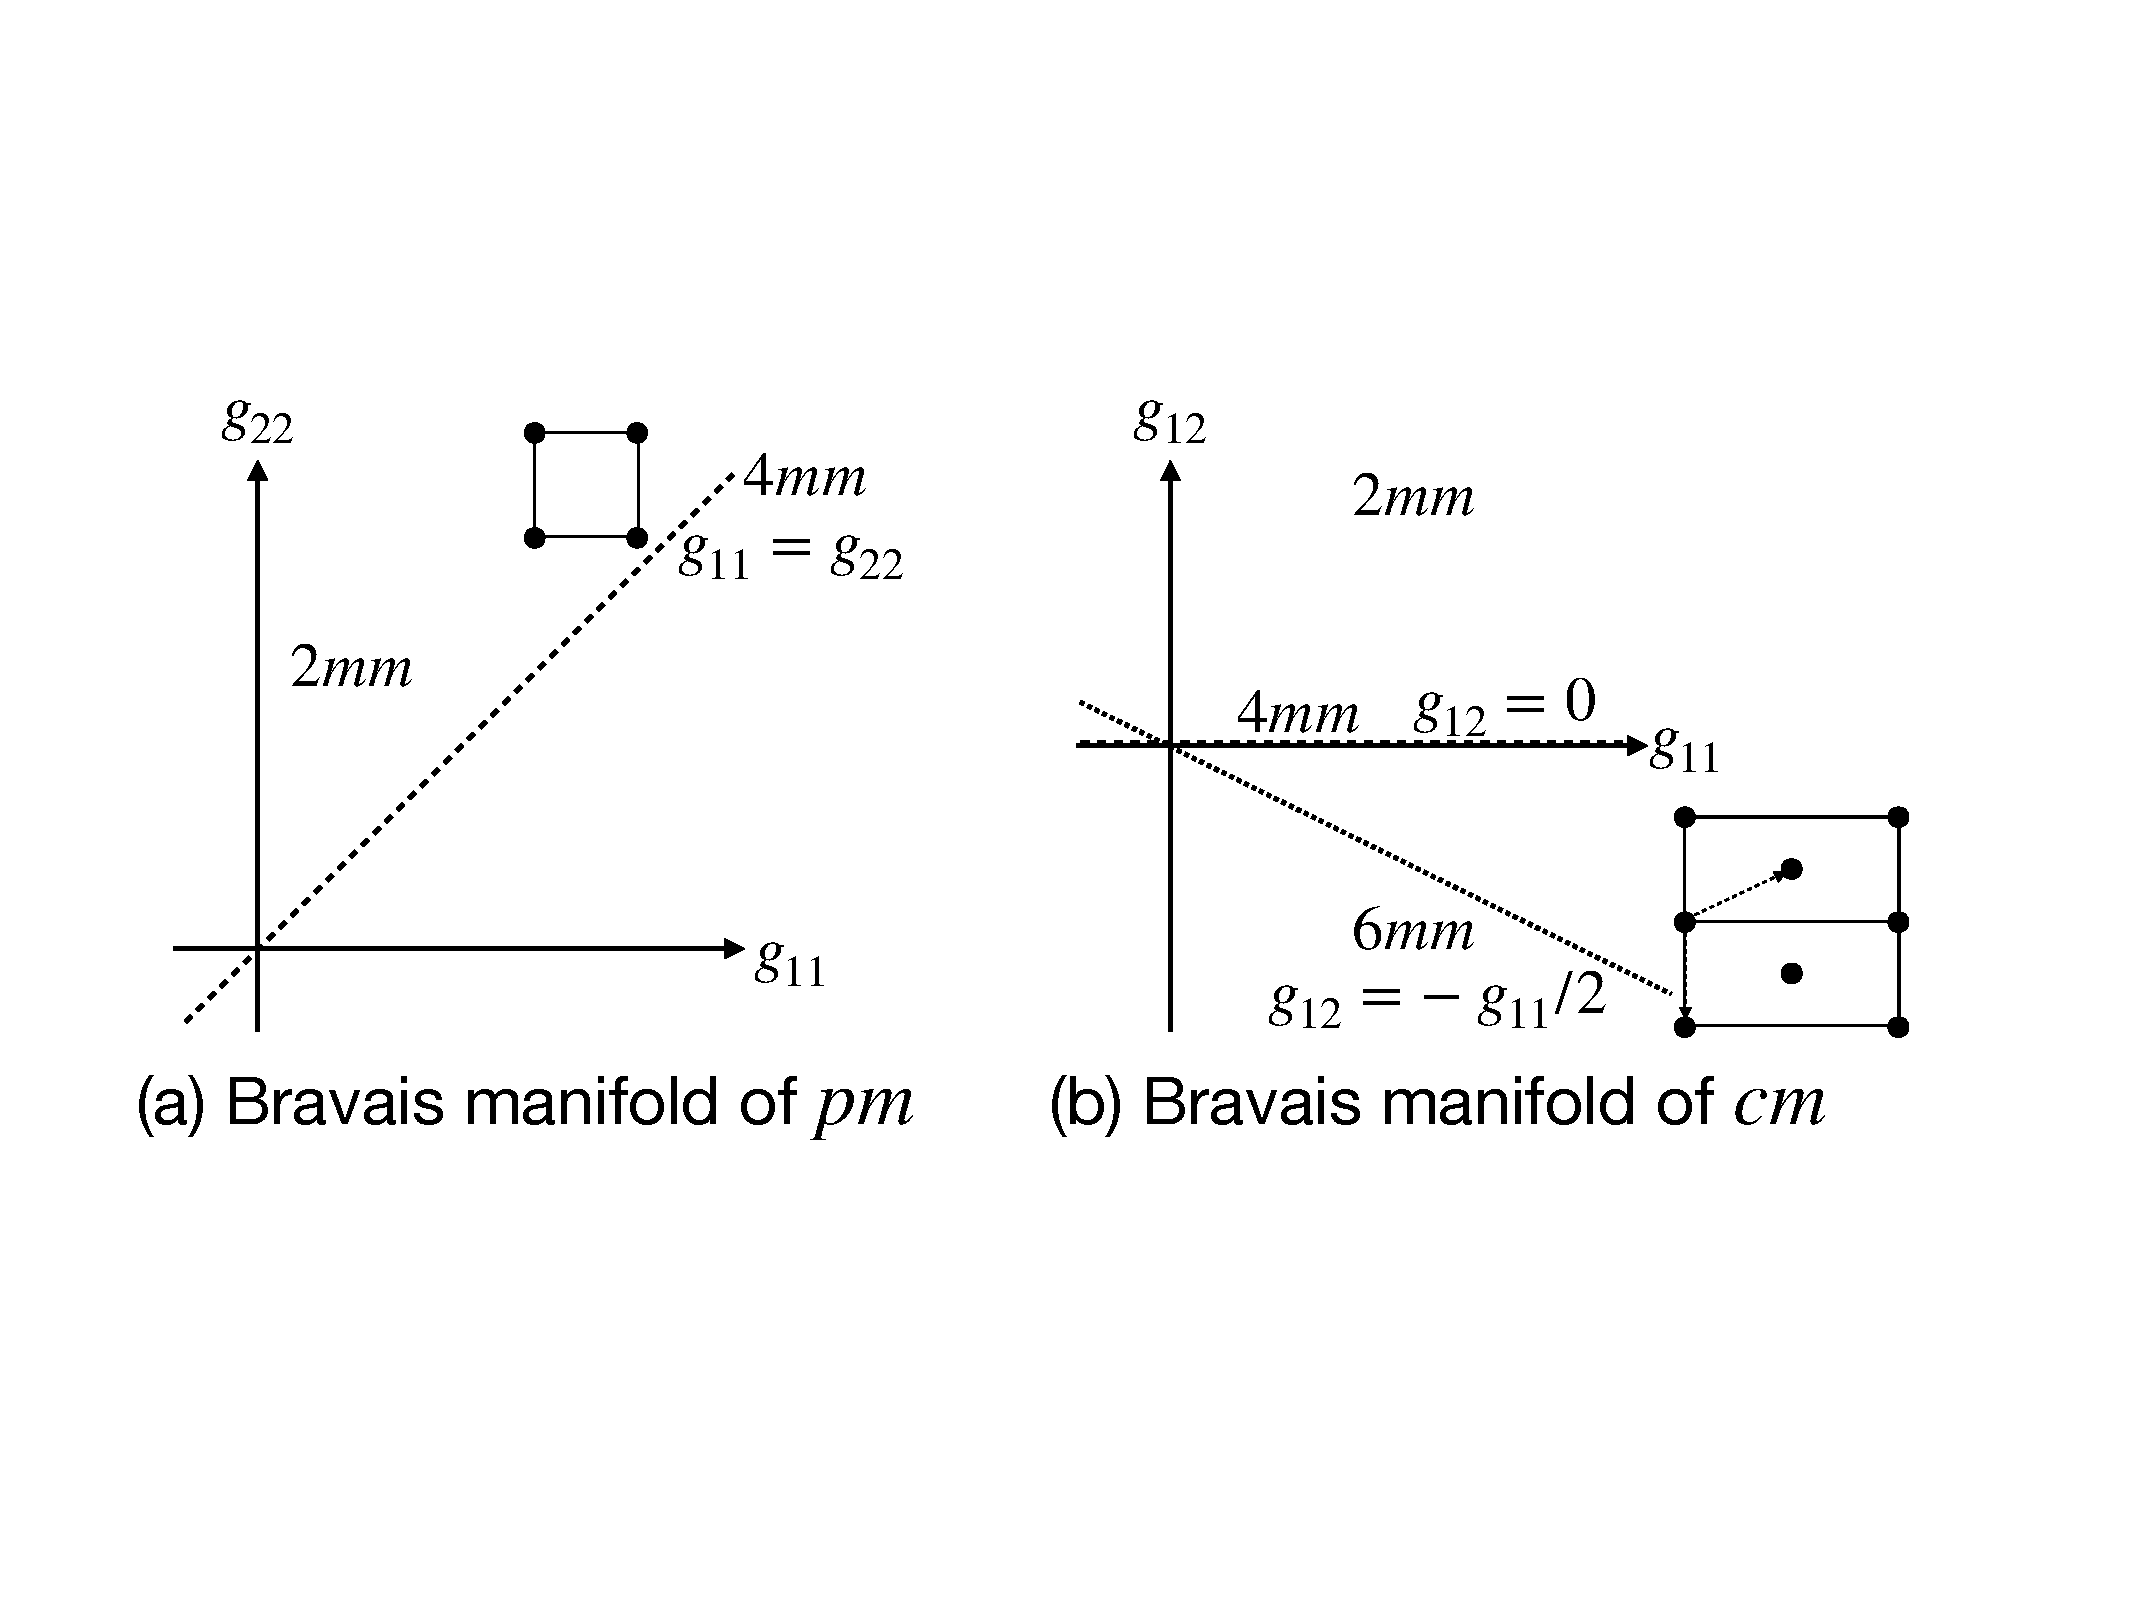
\includegraphics[width=0.9\textwidth]{figure/fig_Bravais_manifold.pdf}
  \caption{Bravais manifolds of point groups of (a) $pm$ and (b) $cm$.}
  \label{fig:bravais_manifold}
\end{figure}

\paragraph{Example: Bravais types of lattices of translation lattices of $pm$ and $cm$}

We consider a translation lattice of $pm$.
We assume cell parameters $a$ and $b$ have no relationship to each other.
The metric tensor for one of the choices of primitive basis vectors is
\begin{align*}
  \bm{G}_{pm} = \begin{pmatrix} a^{2} & 0 \\ 0 & b^{2} \end{pmatrix}.
\end{align*}
The Bravais group of $L_{pm}$ is
\begin{align}
  \label{eq:bravais_group_pm_general}
  \mathcal{B}(L_{pm}) = \left\{
    \begin{pmatrix} 1 & 0 \\ 0 & 1 \\ \end{pmatrix},
    \begin{pmatrix} -1 & 0 \\ 0 & -1 \\ \end{pmatrix},
    \begin{pmatrix} 1 & 0 \\ 0 & -1 \\ \end{pmatrix},
    \begin{pmatrix} -1 & 0 \\ 0 & 1 \\ \end{pmatrix}
  \right\}.
\end{align}

Next, we consider a translation lattice of $cm$, $L_{cm}$.
We transform a conventional cell with cell parameter $\gamma = 90^{\circ}$ to a primitive cell by $(\bm{a}_{p}, \bm{b}_{p}) = (\bm{a}, \bm{b}) \bm{P}$ with
\begin{align*}
  \bm{P} = \frac{1}{2} \begin{pmatrix} 1 & 1 \\ -1 & 1 \end{pmatrix}.
\end{align*}
The metric tensor with the primitive basis vectors is
\begin{align*}
  \bm{G}_{cm} = \begin{pmatrix}
    \frac{a^{2} + b^{2}}{2} & \frac{a^{2} - b^{2}}{2} \\
    \frac{a^{2} - b^{2}}{2} & \frac{a^{2} + b^{2}}{2} \\
  \end{pmatrix}.
\end{align*}
The Bravais group of $L_{cm}$ with the primitive basis vectors is
\begin{align}
  \label{eq:bravais_group_cm_general}
  \mathcal{B}(L_{cm}) = \left\{
    \begin{pmatrix} 1 & 0 \\ 0 & 1 \\ \end{pmatrix},
    \begin{pmatrix} -1 & 0 \\ 0 & -1 \\ \end{pmatrix},
    \begin{pmatrix} 0 & 1 \\ 1 & 0 \\ \end{pmatrix},
    \begin{pmatrix} 0 & -1 \\ -1 & 0 \\ \end{pmatrix}
  \right\}.
\end{align}
The two Bravais groups $\mathcal{B}(L_{pm})$ and $\mathcal{B}(L_{cm})$ are conjugate by $\frac{\pi}{4}$ rotation, which does not belong to $\mathrm{SL}(3, \mathbb{Z})$.
Thus, $L_{pm}$ and $L_{cm}$ belong to the different Bravais types of lattices ($op$ and $oc$).
The Bravais groups for two-dimensional lattices are given in Table~\ref{tab:two-dimensional-Bravais-groups}.

\begin{table}[htb]
  \centering
  \caption{The Bravais groups of two-dimensional lattices (Table~1.3.3.1 of Ref.~\cite{ITA2016})}
  \label{tab:two-dimensional-Bravais-groups}
  \begin{tabular}{ccc}
    \hline\hline
    Lattice & Metric tensor & Bravais group \\ \hline
    oblique & $\begin{pmatrix} g_{11} & g_{12} \\ g_{12} & g_{22} \end{pmatrix}$ & $2$ \\
    rectangular & $\begin{pmatrix} g_{11} & 0 \\ 0 & g_{22} \end{pmatrix}$ & $2mm$ \\
    square & $\begin{pmatrix} g_{11} & 0 \\ 0 & g_{11} \end{pmatrix}$ & $4mm$ \\
    hexagonal & $\begin{pmatrix} g_{11} & -\frac{1}{2} g_{11} \\ -\frac{1}{2} g_{11} & g_{11} \end{pmatrix}$ & $6mm$ \\
    \hline\hline
  \end{tabular}
\end{table}

\subsubsection{Bravais type of lattice and Bravais class}

\begin{screen}
  \begin{defn}[Bravais manifold]
    Let $K$ be a subgroup of $\mathrm{GL}(3, \mathbb{Z})$.
    A \term{space of metric tensors (Bravais manifold) of $K$} is the space of all metric tensors invariant with $K$,
    \begin{align}
      \bm{M}( K ) \coloneqq \set{ \bm{G} \in \mathbb{R}^{3 \times 3}_{\mathrm{sym}} }{ \bm{W}^{\top}\bm{G}\bm{W} = \bm{G} \quad (\forall \bm{W} \in K ) },
    \end{align}
    where $\mathbb{R}^{n \times n}_{\mathrm{sym}}$ is a set of $n \times n$ symmetric real matrices.
  \end{defn}
\end{screen}

Let $L$ and $\mathcal{P}$ be a translation lattice and a point group of a space group $\mathcal{G}$, respectively.
When the dimension of $\bm{M}(\mathcal{B}(L))$ is smaller than that of $\bm{M}(\mathcal{P})$, the translation lattice $L$ is called to have \term{spaciealized metric}.

\begin{screen}
  \begin{defn}[Bravais class]
    Let $L$ be some lattice with a metric tensor $\bm{G}$.
    A space group $\mathcal{G}$ with a point group $\mathcal{P}$ belongs to a \term{Bravais class} corresponding to the Bravais type of $L$ if $\bm{M}(\mathcal{P})$ and $\bm{M}(\mathcal{B}(L))$ are conjugate by some unimodular matrix $\bm{P} \in \mathrm{SL}(3, \mathbb{Z})$ such that $\bm{P}^{\top} \bm{M}(\mathcal{P}) \bm{P} = \bm{M}(\mathcal{B}(L))$.
  \end{defn}
\end{screen}

Note that the definition of Bravais classes is independent of whether a translation lattice is a specialized metric or not.

\begin{screen}
  \begin{defn}[holohedry]
    A subgroup $\mathcal{P}$ of $\mathrm{GL}(3, \mathbb{Z})$ is called \term{holohedry} if there is a lattice $L$ whose Bravais group belongs to the same geometric crystal class of $\mathcal{P}$.
  \end{defn}
\end{screen}

The seven holohedries for the three-dimensional lattices are shown in Table.~\ref{tab:lattice_system}.

\begin{screen}
  \begin{defn}[Bravais arithmetic crystal class]
    The arithmetic crystal class of a space group $\mathcal{G}$ is called a \term{Bravais arithmetic crystal class} if the point group of $\mathcal{G}$ is the Bravais group of the translation lattice $L$ of $\mathcal{G}$,
    \begin{align}
      \mathcal{P} = \mathcal{B}(L).
    \end{align}
  \end{defn}
\end{screen}

Note that Bravais arithmetic crystal classes are classifications for arithmetic crystal classes of space groups, and Bravais classes are classifications for space groups.
The definition of Bravais arithmetic crystal classes is compatible with that of Bravais types of lattices (see Table~\ref{table:arithmetic-class-3d}).

\begin{table}[htb]
  \centering
  \caption{The correspondence of Bravais arithmetic crystal classes and Bravais types of lattices in three dimensions.}
  \label{table:arithmetic-class-3d}
  \begin{tabular}{cc}
    \hline\hline
    Bravais type of lattice & Bravais arithmetic crystal class \\ \hline
    $aP$                    & $\overline{1}P$                  \\
    $mP$                    & $2/mP$                           \\
    $mC$                    & $2/mC$                           \\
    $oP$                    & $mmmP$                           \\
    $oS$                    & $mmmC$                           \\
    $oF$                    & $mmmF$                           \\
    $oI$                    & $mmmI$                           \\
    $tP$                    & $4/mmmP$                         \\
    $tI$                    & $4/mmmI$                         \\
    $hR$                    & $\overline{3}mR$                 \\
    $hP$                    & $6/mmmP$                         \\
    $cP$                    & $m\overline{3}mP$                \\
    $cF$                    & $m\overline{3}mF$                \\
    $cI$                    & $m\overline{3}mI$                \\
    \hline\hline
  \end{tabular}
\end{table}

\paragraph{Example: Bravais manifolds and Bravais classes of $pm$}

The Bravais manifold of the Bravais group in Eq.~\eqref{eq:bravais_group_pm_general} is
\begin{align*}
  \bm{M}(\mathcal{B}(L_{pm})) = \set{
    \begin{pmatrix} g_{11} & 0 \\ 0 & g_{22} \end{pmatrix}
  }{
    g_{11}, g_{22} \in \mathbb{R}
  }.
\end{align*}
If the metric tensor satisfies $g_{11} = g_{22} \, (a = b)$ , the corresponding Bravais group is $4mm$.
The Bravais manifold of $4mm$ has only one free parameter.
Thus, such a lattice has a specialized metric.

The Bravais manifold of the point group of $pm$ is
\begin{align*}
  \bm{M}(\mathcal{P}_{pm}) = \set{
    \begin{pmatrix} g_{11} & 0 \\ 0 & g_{22} \end{pmatrix}
  }{
    g_{11}, g_{22} \in \mathbb{R}
  }.
\end{align*}
Therefore, $pm$ belongs to the Bravais group $op$ whether its translation lattice has a specialized metric or not.

\paragraph{Example: Bravais manifolds and Bravais classes of $cm$}

The Bravais manifold of the Bravais group in Eq.~\eqref{eq:bravais_group_cm_general} is
\begin{align*}
  \bm{M}(\mathcal{B}(L_{cm})) = \set{
    \begin{pmatrix} g_{11} & g_{12} \\ g_{12} & g_{11} \end{pmatrix}
  }{
    g_{11}, g_{12} \in \mathbb{R}
  }.
\end{align*}
If $g_{12} = 0 \, (a = b)$, the corresponding Bravais group is $4mm$.
If $g_{12} = -\frac{1}{2} g_{11} \, (b = \sqrt{3} a)$, the corresponding Bravais group is $6mm$.

The Bravais manifold of the point group of $cm$ is
\begin{align*}
  \bm{M}(\mathcal{P}_{pm}) = \set{
    \begin{pmatrix} g_{11} & 0 \\ 0 & g_{22} \end{pmatrix}
  }{
    g_{11}, g_{22} \in \mathbb{R}
  }.
\end{align*}
Therefore, $cm$ belongs to the Bravais group $oc$ whether its translation lattice has a specialized metric or not.

\subsection{Other classifications}

\subsubsection{\label{sec:lattice-system}Lattice system}

Next, we consider classifying the Bravais classes by ignoring centerings.
\begin{screen}
  \begin{defn}[lattice system]
    Two lattices $L$ and $L'$ belong to the same \term{lattice system} if their Bravais groups belong to the same geometric crystal class, that is, some invertible matrix $\bm{P} \in \mathrm{SL}(3, \mathbb{R})$ exists such that $\bm{P}^{-1} \mathcal{B}(L) \bm{P} = \mathcal{B}(L')$.
  \end{defn}
\end{screen}

Two Bravais classes belong to the same \term{lattice system} if the corresponding Bravais arithmetic crystal classes belong to the same holohedry.
There are seven lattice systems for three-dimensional space groups as shown in Table~\ref{tab:lattice_system}.

\begin{table}[htb]
  \centering
  \caption{Lattice systems in the three-dimensional space}
  \label{tab:lattice_system}
  \begin{tabular}[h]{ccc}
    \hline\hline
    Lattice system & Holohedry & Bravias types of lattices \\ \hline
    Triclinic    & $\overline{1}$   & $aP$                   \\
    Monoclinic   & $2/m$            & $mP$, $mS$             \\
    Orthorhombic & $mmm$            & $oP$, $oS$, $oF$, $oI$ \\
    Tetragonal   & $4/mmm$          & $tP$, $tI$             \\
    Rhombohedral & $\overline{3}m$  & $hR$                   \\
    Hexagonal    & $6/mmm$          & $hP$                   \\
    Cubic        & $m\overline{3}m$ & $cP$, $cF$, $cI$       \\
    \hline\hline
  \end{tabular}
\end{table}

\subsubsection{\label{sec:crystal-system}Crystal system}

\begin{screen}
  \begin{defn}[crytal system]
    Two space groups with point groups $\mathcal{P}$ and $\mathcal{P}'$ belong to the same \term{crystal system} if and only if the sets of Bravais type of lattices on which these point groups act coincide.
  \end{defn}
\end{screen}

There are seven crystal systems for three-dimensional space groups as shown in Table~\ref{tab:crystal_system}.

\begin{table}[htb]
  \centering
  \caption{Crystal systems in space groups}
  \label{tab:crystal_system}
  \begin{tabular}{cc}
    \hline\hline
    Crystal system & Geometric crystal classes                                \\ \hline
    Triclinic      & $1, \overline{1}$                                        \\
    Monoclinic     & $2/m, m, 2$                                              \\
    Orthorhombic   & $mmm, mm2, 222$                                          \\
    Tetragonal     & $4/mmm, \overline{4}2m, 4mm, 422, 4/m, \overline{4}, 4$  \\
    Trigonal       & $\overline{3}m, 3m, 32, \overline{3}, 3$                 \\
    Hexagonal      & $6/mmm, \overline{6}2m, 6mm, 622, 6/m, \overline{6}, 6$  \\
    Cubic          & $m\overline{3}m, \overline{4}3m, 432, m\overline{3}, 23$ \\
    \hline\hline
  \end{tabular}
\end{table}

\subsubsection{\label{sec:crystal-family}Crystal family}

\begin{screen}
  \begin{defn}[crystal family]
    The \term{crystal family} of space group $\mathcal{G}$ is the union of all geometric crystal classes that contain some space group $\mathcal{G}'$ that has the same Bravais type of lattices as $\mathcal{G}$ with the same number of dimensions of Bravais manifolds.
  \end{defn}
\end{screen}

The hexagonal and trigonal crystal systems belong to the same crystal family, called the hexagonal crystal family, because a translation lattice of a trigonal space group with a specialized metric can have the Bravais group, $6/mmm$.
There are six crystal families for the three-dimensional space groups: triclinic, monoclinic, orthorhombic, tetragonal, hexagonal, and cubic.
Also, the hexagonal crystal family is shown in Table~\ref{tab:hexagonal_crystal_family}.

\begin{table}[htb]
  \centering
  \caption{Arithmetic crystal classes belonging to the hexagonal crystal family.}
  \label{tab:hexagonal_crystal_family}
  \begin{tabular}{c|c|c}
    \hline
      Crystal system \textbackslash Lattice system & Hexagonal & Rhombohedral \\ \hline
      Hexagonal & $6/mmmP$, $\overline{6}m2P$, $6mmP$,  & \\
                & $622P$, $6/mP$, $\overline{6}P$, $6P$ & \\ \hline
      Trigonal  & $\overline{3}mP$, $3mP$, $32P$, $\overline{3}P$, $3P$ & $\overline{3}mR$, $3mR$, $32R$, $\overline{3}R$, $3R$ \\
    \hline
  \end{tabular}
\end{table}
